\documentclass[]{article}
\usepackage{lmodern}
\usepackage{amssymb,amsmath}
\usepackage{ifxetex,ifluatex}
\usepackage{fixltx2e} % provides \textsubscript
\ifnum 0\ifxetex 1\fi\ifluatex 1\fi=0 % if pdftex
  \usepackage[T1]{fontenc}
  \usepackage[utf8]{inputenc}
\else % if luatex or xelatex
  \ifxetex
    \usepackage{mathspec}
  \else
    \usepackage{fontspec}
  \fi
  \defaultfontfeatures{Ligatures=TeX,Scale=MatchLowercase}
\fi
% use upquote if available, for straight quotes in verbatim environments
\IfFileExists{upquote.sty}{\usepackage{upquote}}{}
% use microtype if available
\IfFileExists{microtype.sty}{%
\usepackage{microtype}
\UseMicrotypeSet[protrusion]{basicmath} % disable protrusion for tt fonts
}{}
\usepackage[margin=1in]{geometry}
\usepackage{hyperref}
\hypersetup{unicode=true,
            pdftitle={Lab1},
            pdfborder={0 0 0},
            breaklinks=true}
\urlstyle{same}  % don't use monospace font for urls
\usepackage{color}
\usepackage{fancyvrb}
\newcommand{\VerbBar}{|}
\newcommand{\VERB}{\Verb[commandchars=\\\{\}]}
\DefineVerbatimEnvironment{Highlighting}{Verbatim}{commandchars=\\\{\}}
% Add ',fontsize=\small' for more characters per line
\usepackage{framed}
\definecolor{shadecolor}{RGB}{248,248,248}
\newenvironment{Shaded}{\begin{snugshade}}{\end{snugshade}}
\newcommand{\AlertTok}[1]{\textcolor[rgb]{0.94,0.16,0.16}{#1}}
\newcommand{\AnnotationTok}[1]{\textcolor[rgb]{0.56,0.35,0.01}{\textbf{\textit{#1}}}}
\newcommand{\AttributeTok}[1]{\textcolor[rgb]{0.77,0.63,0.00}{#1}}
\newcommand{\BaseNTok}[1]{\textcolor[rgb]{0.00,0.00,0.81}{#1}}
\newcommand{\BuiltInTok}[1]{#1}
\newcommand{\CharTok}[1]{\textcolor[rgb]{0.31,0.60,0.02}{#1}}
\newcommand{\CommentTok}[1]{\textcolor[rgb]{0.56,0.35,0.01}{\textit{#1}}}
\newcommand{\CommentVarTok}[1]{\textcolor[rgb]{0.56,0.35,0.01}{\textbf{\textit{#1}}}}
\newcommand{\ConstantTok}[1]{\textcolor[rgb]{0.00,0.00,0.00}{#1}}
\newcommand{\ControlFlowTok}[1]{\textcolor[rgb]{0.13,0.29,0.53}{\textbf{#1}}}
\newcommand{\DataTypeTok}[1]{\textcolor[rgb]{0.13,0.29,0.53}{#1}}
\newcommand{\DecValTok}[1]{\textcolor[rgb]{0.00,0.00,0.81}{#1}}
\newcommand{\DocumentationTok}[1]{\textcolor[rgb]{0.56,0.35,0.01}{\textbf{\textit{#1}}}}
\newcommand{\ErrorTok}[1]{\textcolor[rgb]{0.64,0.00,0.00}{\textbf{#1}}}
\newcommand{\ExtensionTok}[1]{#1}
\newcommand{\FloatTok}[1]{\textcolor[rgb]{0.00,0.00,0.81}{#1}}
\newcommand{\FunctionTok}[1]{\textcolor[rgb]{0.00,0.00,0.00}{#1}}
\newcommand{\ImportTok}[1]{#1}
\newcommand{\InformationTok}[1]{\textcolor[rgb]{0.56,0.35,0.01}{\textbf{\textit{#1}}}}
\newcommand{\KeywordTok}[1]{\textcolor[rgb]{0.13,0.29,0.53}{\textbf{#1}}}
\newcommand{\NormalTok}[1]{#1}
\newcommand{\OperatorTok}[1]{\textcolor[rgb]{0.81,0.36,0.00}{\textbf{#1}}}
\newcommand{\OtherTok}[1]{\textcolor[rgb]{0.56,0.35,0.01}{#1}}
\newcommand{\PreprocessorTok}[1]{\textcolor[rgb]{0.56,0.35,0.01}{\textit{#1}}}
\newcommand{\RegionMarkerTok}[1]{#1}
\newcommand{\SpecialCharTok}[1]{\textcolor[rgb]{0.00,0.00,0.00}{#1}}
\newcommand{\SpecialStringTok}[1]{\textcolor[rgb]{0.31,0.60,0.02}{#1}}
\newcommand{\StringTok}[1]{\textcolor[rgb]{0.31,0.60,0.02}{#1}}
\newcommand{\VariableTok}[1]{\textcolor[rgb]{0.00,0.00,0.00}{#1}}
\newcommand{\VerbatimStringTok}[1]{\textcolor[rgb]{0.31,0.60,0.02}{#1}}
\newcommand{\WarningTok}[1]{\textcolor[rgb]{0.56,0.35,0.01}{\textbf{\textit{#1}}}}
\usepackage{graphicx}
% grffile has become a legacy package: https://ctan.org/pkg/grffile
\IfFileExists{grffile.sty}{%
\usepackage{grffile}
}{}
\makeatletter
\def\maxwidth{\ifdim\Gin@nat@width>\linewidth\linewidth\else\Gin@nat@width\fi}
\def\maxheight{\ifdim\Gin@nat@height>\textheight\textheight\else\Gin@nat@height\fi}
\makeatother
% Scale images if necessary, so that they will not overflow the page
% margins by default, and it is still possible to overwrite the defaults
% using explicit options in \includegraphics[width, height, ...]{}
\setkeys{Gin}{width=\maxwidth,height=\maxheight,keepaspectratio}
\IfFileExists{parskip.sty}{%
\usepackage{parskip}
}{% else
\setlength{\parindent}{0pt}
\setlength{\parskip}{6pt plus 2pt minus 1pt}
}
\setlength{\emergencystretch}{3em}  % prevent overfull lines
\providecommand{\tightlist}{%
  \setlength{\itemsep}{0pt}\setlength{\parskip}{0pt}}
\setcounter{secnumdepth}{0}
% Redefines (sub)paragraphs to behave more like sections
\ifx\paragraph\undefined\else
\let\oldparagraph\paragraph
\renewcommand{\paragraph}[1]{\oldparagraph{#1}\mbox{}}
\fi
\ifx\subparagraph\undefined\else
\let\oldsubparagraph\subparagraph
\renewcommand{\subparagraph}[1]{\oldsubparagraph{#1}\mbox{}}
\fi

%%% Use protect on footnotes to avoid problems with footnotes in titles
\let\rmarkdownfootnote\footnote%
\def\footnote{\protect\rmarkdownfootnote}

%%% Change title format to be more compact
\usepackage{titling}

% Create subtitle command for use in maketitle
\providecommand{\subtitle}[1]{
  \posttitle{
    \begin{center}\large#1\end{center}
    }
}

\setlength{\droptitle}{-2em}

  \title{Lab1}
    \pretitle{\vspace{\droptitle}\centering\huge}
  \posttitle{\par}
    \author{}
    \preauthor{}\postauthor{}
    \date{}
    \predate{}\postdate{}
  

\begin{document}
\maketitle

\hypertarget{computer-lab-1}{%
\subsection{Computer Lab 1}\label{computer-lab-1}}

\hypertarget{assignment-1}{%
\section{Assignment 1}\label{assignment-1}}

*(1a)

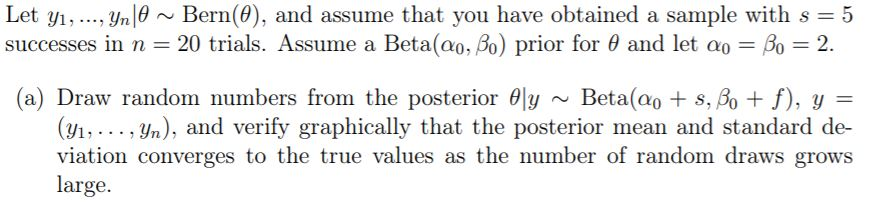
\includegraphics[width=0.6\linewidth]{1a}

As n gets bigger the mean and standard deviation converges towards its
true value. Bigger amount of data (n) results in that the prior has less
influence on the posterior. Mean -\textgreater{} 0,29 st -\textgreater{}
0,09

\includegraphics{Bayesian_Lab1_files/figure-latex/1a-1.pdf}
\includegraphics{Bayesian_Lab1_files/figure-latex/1a-2.pdf}

\emph{(b) Use simulation (nDraws = 10000) to compute the posterior
probability} \emph{Pr(theta \textgreater{} 0.3\textbar y) and compare
with the exact value {[}Hint: pbeta(){]}.}

When similating nDraws = 10000 and counting the cases where the
estimated probablity is bigger than 0,3 we see that the value is fairly
close to the true value given the data y. Depening on the amount of
draws we see that the posterior probaliblity for theta\textgreater0,3
given the data will be closer and closer to the true value.

\begin{verbatim}
## [1] 0.4389
\end{verbatim}

\begin{verbatim}
## [1] 0.4399472
\end{verbatim}

\emph{c) Compute the posterior distribution of the log-odds phi =
log(phu / (1-phi) by simulation (nDraws = 10000). {[}Hint: hist() and
density() might come in handy{]}}

The log-odds posterior distribution can be seen in the plot. It looks
like the same distribution as the data of shown in histogram.

\includegraphics{Bayesian_Lab1_files/figure-latex/1c-1.pdf}
\includegraphics{Bayesian_Lab1_files/figure-latex/1c-2.pdf}

\hypertarget{assignment-2}{%
\section{Assignment 2}\label{assignment-2}}

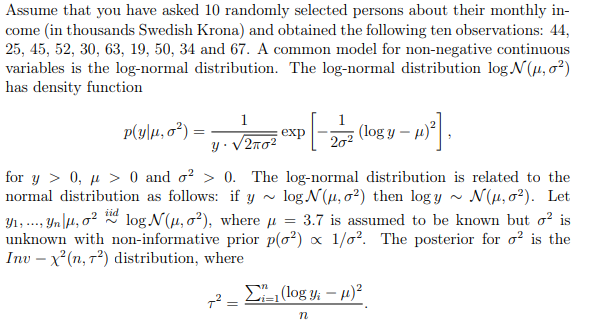
\includegraphics[width=0.6\linewidth]{Capture}
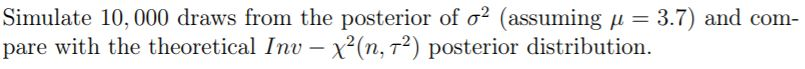
\includegraphics[width=0.6\linewidth]{2a}

\emph{(2a)}

We simulated a distribution from the posterior by drawing 10000 values
and using density() to get the distribution. We are aware that density()
only fits the data and does not yield the true distribution, but since n
is so big (10000) we believe that density() will fit the model
realisticly. Using density makes it easier to compare distribution than
if we would use a histogram. We compared this distribution with the
theoretical distribution and found that they were almost identical.

\includegraphics{Bayesian_Lab1_files/figure-latex/2a-1.pdf}

\emph{2b)} \emph{Use the posterior draws in a) to compute the posterior
distribution of the Gini coefficient G for the current data set.}

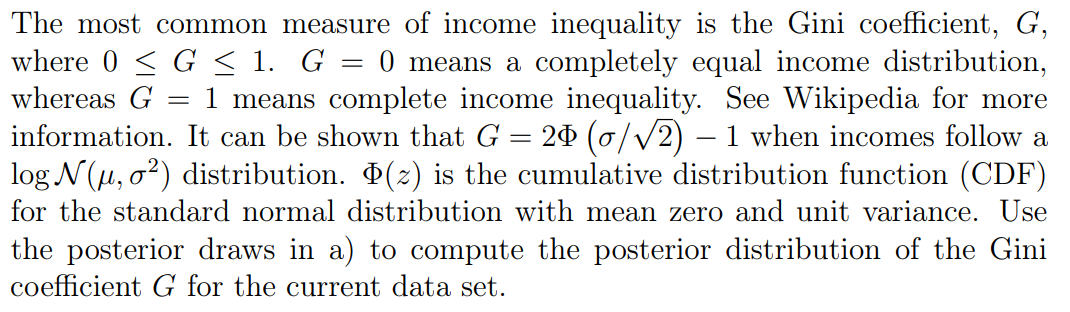
\includegraphics[width=0.6\linewidth]{2b}
\includegraphics[width=0.6\linewidth]{Bayesian_Lab1_files/figure-latex/2b-2}

When plotting the posterior distribution of the Gini Coefficients we can
observe that it is very similar to the plot of the posterior
distribution sigma\^{}2. It is reasonable that the distribution is
similar since the Gini Coeffiecients is just a transfromaion of the
sigma\^{}2, since the income has a conjugate prior which is scaled
inverse chi-squared.

\emph{2c)}

\emph{Use the posterior draws from b) to compute a 90\% equal tail
credible interval for G. A 90\% equal tail interval (a, b) cuts off 5\%
percent of the posterior probability mass to the left of a, and 5\% to
the right of b. Also, do a kernel density estimate of the posterior of G
using the density function in R with default settings, and use that
kernel density estimate to compute a 90\% Highest Posterior Density
interval for G. Compare the two intervals}

We obtained a credible interval of (0.046,0.21) and a highest posterior
density interval of (0.33,0.176). We used the default kernel (Gaussian)
with the default bandwidth for the HDI. In symmetric distributions,
credible interval and HDI will return same results. With skewed
distributions such as this one the HDI will move to the more probable
values while credible interval is limited to the 5 and 95 percentile.
Since the HDI covers more probable values we believe that this interval
seems to be a more intuitive and meaningful summary of the posterior.

\begin{verbatim}
## Warning: package 'HDInterval' was built under R version 3.6.3
\end{verbatim}

\hypertarget{assignment-3}{%
\section{Assignment 3}\label{assignment-3}}

\emph{(3a) Plot the posterior distribution of κ for the wind direction
data over a fine grid of κ value}

The posterior distribution of k is obtained through the proportinality
on likelihood vector of y\textbar k multiplied by probability
distribution p(k). Since the prior distribution of k is given the
probability vector of k can be calculated. The likelihood vector of
y\textbar k is obtained by feeding the given likelihood function with
the k values used to create the probability vector of k. By the final
mltiplikation likelilhood(y\textbar k)*p(k) we the get the posterior
density for all values of k.

p(k\textbar y) proportial to p(y\textbar k)*p(k)

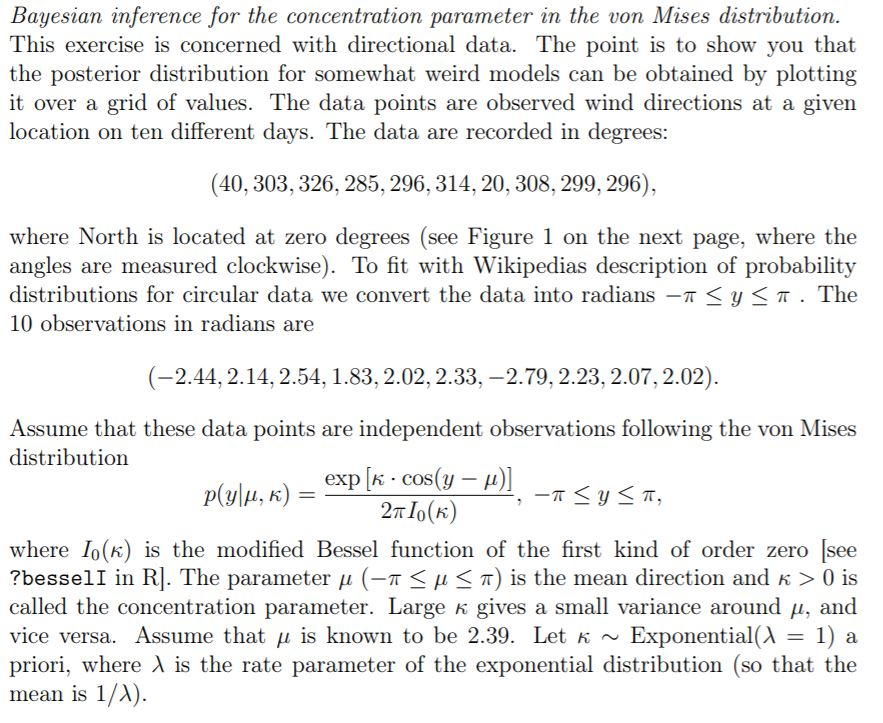
\includegraphics[width=0.6\linewidth]{3a}
\includegraphics[width=0.6\linewidth]{Bayesian_Lab1_files/figure-latex/3a-2}

\emph{(b)Find the(approximate) posterior mode of κ from the information
in a)}

By finding the maximum value of the density and extracting its index we
can then get the k value which results in the highest probability

\begin{Shaded}
\begin{Highlighting}[]
\CommentTok{# Bernoulli ... again.}
\CommentTok{# Let y1, ..., yn|?? ??? Bern(??), and assume that you have obtained a sample with s = 5}
\CommentTok{# successes in n = 20 trials. Assume a Beta(??0, ??0) prior for ?? and let ??0 = ??0 = 2.}

\CommentTok{# a)}
\CommentTok{# Draw random numbers from the posterior ??|y ??? Beta(??0 + s, ??0 + f), y = (y1, . . . , yn), }
\CommentTok{# and verify graphically that the posterior mean and standard deviation}
\CommentTok{# converges to the true values as the number of random draws grows large.}

\NormalTok{vec =}\StringTok{ }\KeywordTok{c}\NormalTok{()}
\NormalTok{deviation =}\StringTok{ }\KeywordTok{c}\NormalTok{()}
\NormalTok{number =}\StringTok{ }\KeywordTok{c}\NormalTok{()}

\CommentTok{# Prior}
\NormalTok{a =}\StringTok{ }\NormalTok{b =}\StringTok{ }\DecValTok{2}
\NormalTok{s =}\StringTok{ }\DecValTok{5}
\NormalTok{n =}\StringTok{ }\DecValTok{20}
\NormalTok{f =}\StringTok{ }\NormalTok{n}\OperatorTok{-}\NormalTok{s}

\CommentTok{# Posterior}
\NormalTok{posterior_alpha =}\StringTok{ }\NormalTok{s }\OperatorTok{+}\StringTok{ }\NormalTok{a}
\NormalTok{posterior_beta =}\StringTok{ }\NormalTok{b }\OperatorTok{+}\StringTok{ }\NormalTok{f}

\ControlFlowTok{for}\NormalTok{ (i }\ControlFlowTok{in} \DecValTok{1}\OperatorTok{:}\DecValTok{1000}\NormalTok{)\{}
\NormalTok{  post =}\StringTok{ }\KeywordTok{rbeta}\NormalTok{ (i, posterior_alpha, posterior_beta)}
\NormalTok{  mean =}\KeywordTok{mean}\NormalTok{(post)}
\NormalTok{  st =}\StringTok{ }\KeywordTok{sd}\NormalTok{(post)}
\NormalTok{  vec =}\StringTok{ }\KeywordTok{append}\NormalTok{(vec,mean)}
\NormalTok{  deviation =}\StringTok{ }\KeywordTok{append}\NormalTok{(deviation,st)}
\NormalTok{  number =}\StringTok{ }\KeywordTok{append}\NormalTok{(number, i)}
\NormalTok{\}}

\CommentTok{# Plot theta means}
\KeywordTok{plot}\NormalTok{(number, vec, }\DataTypeTok{type=}\StringTok{'l'}\NormalTok{, }\DataTypeTok{xlab=}\StringTok{'Number of draws'}\NormalTok{, }\DataTypeTok{ylab=}\StringTok{'Mean of theta'}\NormalTok{)}

\CommentTok{# Plot theta deviations}
\KeywordTok{plot}\NormalTok{(deviation)}
\KeywordTok{plot}\NormalTok{(number, deviation, }\DataTypeTok{type=}\StringTok{'l'}\NormalTok{, }\DataTypeTok{xlab=}\StringTok{'Number of draws'}\NormalTok{, }\DataTypeTok{ylab=}\StringTok{'deviation'}\NormalTok{)}

\CommentTok{# b)}
\CommentTok{# Use simulation (nDraws = 10000) to compute the posterior probability }
\CommentTok{# Pr(?? > 0.3|y) and compare with the exact value [Hint: pbeta()].}

\NormalTok{draws =}\StringTok{ }\KeywordTok{rbeta}\NormalTok{ (}\DecValTok{10000}\NormalTok{, posterior_alpha, posterior_beta)}
\NormalTok{bigger_than =}\StringTok{ }\KeywordTok{ifelse}\NormalTok{(draws}\OperatorTok{>}\FloatTok{0.3}\NormalTok{,}\DecValTok{1}\NormalTok{,}\DecValTok{0}\NormalTok{)}
\NormalTok{prob_bigger_than =}\StringTok{ }\KeywordTok{sum}\NormalTok{(bigger_than)}\OperatorTok{/}\KeywordTok{length}\NormalTok{(draws)}
\NormalTok{prob_bigger_than}


\NormalTok{theta_bigger_than =}\StringTok{ }\KeywordTok{pbeta}\NormalTok{(}\FloatTok{0.3}\NormalTok{, posterior_alpha, posterior_beta, }\DataTypeTok{ncp =} \DecValTok{0}\NormalTok{, }\DataTypeTok{lower.tail =} \OtherTok{FALSE}\NormalTok{, }\DataTypeTok{log.p =} \OtherTok{FALSE}\NormalTok{)}
\KeywordTok{print}\NormalTok{(theta_bigger_than)}

\CommentTok{# c) }
\CommentTok{# Compute the posterior distribution of the log-odds ?? = log(?? / 1?????)}
\CommentTok{# by simulation (nDraws = 10000). [Hint: hist() and density() might come in handy]}

\NormalTok{logdraws =}\StringTok{ }\KeywordTok{log}\NormalTok{(draws}\OperatorTok{/}\NormalTok{(}\DecValTok{1}\OperatorTok{-}\NormalTok{draws))}
\NormalTok{densityLogDraws =}\StringTok{ }\KeywordTok{density}\NormalTok{(logdraws)}
\KeywordTok{plot}\NormalTok{(densityLogDraws,}
     \DataTypeTok{main =} \StringTok{"Log-odds posterior distribution"}\NormalTok{, }
     \DataTypeTok{ylab =} \StringTok{"Density"}\NormalTok{,}
     \DataTypeTok{xlab =} \StringTok{"phi"}\NormalTok{)}

\KeywordTok{hist}\NormalTok{(logdraws)}

\CommentTok{## ASSIGNEMNT 2}

\CommentTok{# Log-normal distribution and the Gini coefficient.}
\CommentTok{# Assume that you have asked 10 randomly selected persons about their monthly income}
\CommentTok{# (in thousands Swedish Krona) and obtained the following ten observations: 44,}
\CommentTok{# 25, 45, 25, 30, 33, 19, 50, 34 and 67. A common model for non-negative continuous}
\CommentTok{# variables is the log-normal distribution}

\CommentTok{# a)}
\CommentTok{# Simulate 10, 000 draws from the posterior of ??2}
\CommentTok{# (assuming µ = 3.7) and compare with the theoretical }
\CommentTok{# Inv ??? ??2(n, ?? 2) posterior distribution.}

\NormalTok{my =}\StringTok{ }\FloatTok{3.7}
\NormalTok{n =}\StringTok{ }\DecValTok{10}

\NormalTok{Y =}\StringTok{ }\KeywordTok{c}\NormalTok{(}\DecValTok{44}\NormalTok{,}\DecValTok{25}\NormalTok{,}\DecValTok{45}\NormalTok{,}\DecValTok{52}\NormalTok{,}\DecValTok{30}\NormalTok{,}\DecValTok{63}\NormalTok{,}\DecValTok{19}\NormalTok{,}\DecValTok{50}\NormalTok{,}\DecValTok{34}\NormalTok{,}\DecValTok{67}\NormalTok{)}
\CommentTok{#compute sample variance s^2}
\NormalTok{T2 =}\StringTok{  }\KeywordTok{sum}\NormalTok{((}\KeywordTok{log}\NormalTok{(Y)}\OperatorTok{-}\NormalTok{my)}\OperatorTok{^}\DecValTok{2}\NormalTok{)}\OperatorTok{/}\NormalTok{n}

\CommentTok{#Draw X from chi2(n) (This is a draw from Inv- X^2(n,s^2))}
\KeywordTok{set.seed}\NormalTok{(}\DecValTok{12345}\NormalTok{)}
\NormalTok{XposteriorDraw =}\StringTok{ }\KeywordTok{rchisq}\NormalTok{(}\DecValTok{10000}\NormalTok{,}\DecValTok{10}\NormalTok{)}

\CommentTok{# get deviation^2 from X ( deviation^2 = df*s^2 /X)}
\NormalTok{deviationPostDraw =}\StringTok{ }\DecValTok{10}\OperatorTok{*}\NormalTok{T2}\OperatorTok{/}\NormalTok{XposteriorDraw}
\NormalTok{distDeviationPostDraw =}\StringTok{ }\KeywordTok{density}\NormalTok{(deviationPostDraw)}

\KeywordTok{library}\NormalTok{(invgamma)}

\CommentTok{# function for scaled inverse chi-squared pdf}
\NormalTok{invscaledchi2 <-}\StringTok{ }\ControlFlowTok{function}\NormalTok{(x, df, tao2) \{}
\NormalTok{  a <-}\StringTok{ }\NormalTok{df }\OperatorTok{/}\StringTok{ }\DecValTok{2}
\NormalTok{  ((n}\OperatorTok{*}\NormalTok{tao2 }\OperatorTok{/}\StringTok{ }\DecValTok{2}\NormalTok{)}\OperatorTok{^}\NormalTok{a)}\OperatorTok{/}\KeywordTok{gamma}\NormalTok{(a) }\OperatorTok{*}\StringTok{ }\NormalTok{x}\OperatorTok{^}\NormalTok{(}\OperatorTok{-}\NormalTok{a}\DecValTok{-1}\NormalTok{) }\OperatorTok{*}\StringTok{ }\KeywordTok{exp}\NormalTok{(}\OperatorTok{-}\NormalTok{(n}\OperatorTok{*}\NormalTok{tao2 }\OperatorTok{/}\StringTok{ }\DecValTok{2}\NormalTok{)}\OperatorTok{/}\NormalTok{x)}
\NormalTok{\}}


\CommentTok{# sequence of x-values to illustrate the distribution}
\NormalTok{xrange =}\StringTok{ }\KeywordTok{seq}\NormalTok{(}\FloatTok{0.01}\NormalTok{,}\FloatTok{3.0}\NormalTok{,}\FloatTok{0.001}\NormalTok{)}

\CommentTok{# values from inverse chisquared mapped on x-range}
\NormalTok{deviations =}\StringTok{ }\KeywordTok{invscaledchi2}\NormalTok{(xrange,}\DecValTok{10}\NormalTok{,T2)}

\CommentTok{# plot simulated distribution with theoretical distribution}
\KeywordTok{plot}\NormalTok{(distDeviationPostDraw)}
\KeywordTok{lines}\NormalTok{(xrange, deviations, }\DataTypeTok{type=}\StringTok{"l"}\NormalTok{,}\DataTypeTok{col=}\StringTok{"red"}\NormalTok{)}


\CommentTok{# b)}
\CommentTok{# Use}
\CommentTok{#the posterior draws in a) to compute the posterior distribution of the Gini}
\CommentTok{#coefficient G for the current data se}

\CommentTok{#Use draws from posterior to form GiniCoeffient}
\NormalTok{Gini_coefficients =}\StringTok{ }\DecValTok{2}\OperatorTok{*}\KeywordTok{pnorm}\NormalTok{(deviationPostDraw}\OperatorTok{/}\KeywordTok{sqrt}\NormalTok{(}\DecValTok{2}\NormalTok{),}\DecValTok{0}\NormalTok{,}\DecValTok{1}\NormalTok{)}\OperatorTok{-}\DecValTok{1}
\NormalTok{Gini_density =}\StringTok{ }\KeywordTok{density}\NormalTok{(Gini_coefficients)}
\KeywordTok{plot}\NormalTok{(Gini_density, }\DataTypeTok{main =} \StringTok{"Distribution of Gini Coefficients"}\NormalTok{, }\DataTypeTok{xlab =} \StringTok{"Gini Coefficient"}\NormalTok{, }\DataTypeTok{ylab =} \StringTok{"Probability Density"}\NormalTok{)}

\CommentTok{#c}
\CommentTok{#Use the posterior draws from b) to compute a 90% equal tail credible interval}
\CommentTok{#for G. A 90% equal tail interval (a, b) cuts off 5% percent of the posterior}
\CommentTok{#probability mass to the left of a, and 5% to the right of b.}

\NormalTok{GiniQuantiles =}\StringTok{ }\KeywordTok{quantile}\NormalTok{(Gini_coefficients, }\DataTypeTok{probs=}\KeywordTok{seq}\NormalTok{(}\DecValTok{0}\NormalTok{,}\DecValTok{1}\NormalTok{,}\FloatTok{0.05}\NormalTok{))}
\NormalTok{Crediblerange =}\StringTok{ }\KeywordTok{c}\NormalTok{(GiniQuantiles[}\DecValTok{2}\NormalTok{],GiniQuantiles[}\DecValTok{20}\NormalTok{])}
\CommentTok{# gets range (0.046,0.21)}

\CommentTok{#Also, do a kernel density estimate of the posterior of G using the density function in R with}
\CommentTok{#default settings, and use that kernel density estimate to compute a 90% Highest}
\CommentTok{#Posterior Density interval for G. Compare the two intervals}

\CommentTok{# using library from CRAN to get highest (posterior) density interval}
\KeywordTok{library}\NormalTok{(HDInterval)}
\NormalTok{hdiRange =}\StringTok{ }\KeywordTok{hdi}\NormalTok{(Gini_density, }\DataTypeTok{credMass=}\FloatTok{0.9}\NormalTok{)}
\CommentTok{# gets range (0.033,0.176)}

\KeywordTok{hist}\NormalTok{(Gini_coefficients)}
\KeywordTok{plot}\NormalTok{(Gini_density)}


\CommentTok{# Assignment 3}
\CommentTok{# a) }
\CommentTok{# Plot the posterior distribution of ?? for the wind direction data over a fine grid}
\CommentTok{# of ?? values}


\NormalTok{y =}\StringTok{ }\KeywordTok{c}\NormalTok{(}\OperatorTok{-}\FloatTok{2.44}\NormalTok{, }\FloatTok{2.14}\NormalTok{, }\FloatTok{2.54}\NormalTok{, }\FloatTok{1.83}\NormalTok{, }\FloatTok{2.02}\NormalTok{, }\FloatTok{2.33}\NormalTok{, }\FloatTok{-2.79}\NormalTok{, }\FloatTok{2.23}\NormalTok{, }\FloatTok{2.07}\NormalTok{, }\FloatTok{2.02}\NormalTok{)}
\NormalTok{my =}\StringTok{ }\FloatTok{2.39}
\NormalTok{lambda =}\StringTok{ }\DecValTok{1}

\NormalTok{k_prior =}\StringTok{ }\ControlFlowTok{function}\NormalTok{(lambda, k)\{}
\NormalTok{  lambda}\OperatorTok{*}\KeywordTok{exp}\NormalTok{(}\OperatorTok{-}\NormalTok{lambda}\OperatorTok{*}\NormalTok{k) }
\NormalTok{\}}

\NormalTok{likelihood_function =}\StringTok{ }\ControlFlowTok{function}\NormalTok{(k, y, my)\{}
  \KeywordTok{prod}\NormalTok{(}\KeywordTok{exp}\NormalTok{(k}\OperatorTok{*}\KeywordTok{cos}\NormalTok{(y}\OperatorTok{-}\NormalTok{my))}\OperatorTok{/}\NormalTok{(}\DecValTok{2}\OperatorTok{*}\NormalTok{pi}\OperatorTok{*}\KeywordTok{besselI}\NormalTok{(k, }\DecValTok{0}\NormalTok{)))}
\NormalTok{\}}

\NormalTok{sequence =}\StringTok{ }\KeywordTok{seq}\NormalTok{(}\FloatTok{0.1}\NormalTok{, }\DecValTok{5}\NormalTok{, }\FloatTok{0.1}\NormalTok{)}

\NormalTok{k_prior_vector =}\StringTok{ }\KeywordTok{k_prior}\NormalTok{(lambda, sequence)}

\NormalTok{likelihood_vector =}\StringTok{ }\KeywordTok{c}\NormalTok{()}
\NormalTok{test =}\StringTok{ }\KeywordTok{c}\NormalTok{()}
\ControlFlowTok{for}\NormalTok{ (k }\ControlFlowTok{in}\NormalTok{ sequence)\{}
\NormalTok{  likelihood_vector =}\StringTok{ }\KeywordTok{append}\NormalTok{(likelihood_vector, }\KeywordTok{likelihood_function}\NormalTok{(k, y, my))}
\NormalTok{\}}

\NormalTok{k_posterior =}\StringTok{ }\NormalTok{likelihood_vector}\OperatorTok{*}\NormalTok{k_prior_vector}
\KeywordTok{plot}\NormalTok{(sequence, k_posterior, }\DataTypeTok{main =} \StringTok{"Posterior distribution of K"}\NormalTok{, }\DataTypeTok{xlab =} \StringTok{"K"}\NormalTok{, }\DataTypeTok{ylab =} \StringTok{"Density"}\NormalTok{ )}


\CommentTok{# b)}
\CommentTok{# Find the approximate  posterior mode of k  from the information in a}

\NormalTok{k_index =}\StringTok{ }\KeywordTok{which}\NormalTok{(k_posterior }\OperatorTok{==}\StringTok{ }\KeywordTok{max}\NormalTok{(k_posterior))}
\NormalTok{k_mode =}\StringTok{ }\NormalTok{sequence[k_index]}
\end{Highlighting}
\end{Shaded}


\end{document}
